% Frozen PTB-XL Fold 8 (n=2,173 records), Q8/full-lead inputs. PCA is fitted
% separately within each frozen encoder; coordinates are not cross-model aligned.
\begin{figure*}[t]
  \centering
  \includegraphics[width=0.95\textwidth]{figures/frozen_ptbxl_latent_comparison/fig1_fold8_latent_spaces.pdf}
  \caption{Held-out PTB-XL Fold-8 latent spaces for the four frozen encoders.
  Each panel is a separate PCA after within-model feature standardization; hence
  relative point structure, rather than axes, is comparable across panels.
  Colored points carry each superdiagnostic label (labels are non-exclusive);
  gray points provide the full record distribution.}
  \label{fig:frozen-fold8-latents}
\end{figure*}

\begin{figure}[t]
  \centering
  \includegraphics[width=0.48\textwidth]{figures/frozen_ptbxl_latent_comparison/fig2_fold8_latent_spectrum.pdf}
  \caption{Cumulative PCA variance of the frozen Fold-8 latents after
  within-model feature standardization. This describes representation
  concentration; it is not a diagnostic-performance comparison.}
  \label{fig:frozen-fold8-spectrum}
\end{figure}

\begin{figure*}[t]
  \centering
  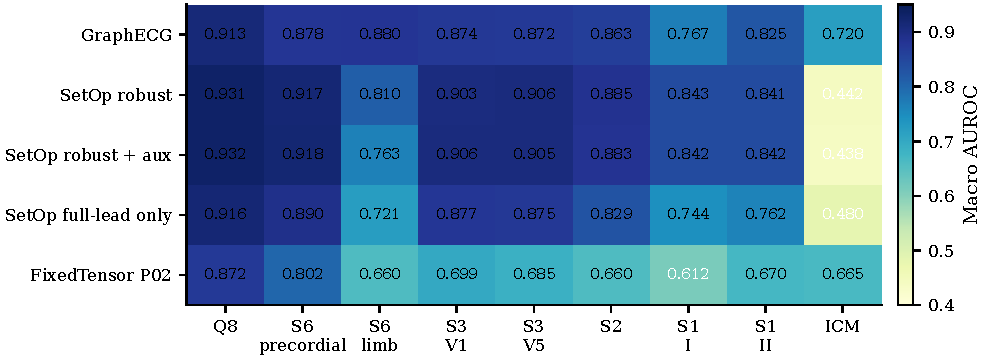
\includegraphics[width=0.95\textwidth]{figures/frozen_ptbxl_latent_comparison/fig3_ptbxl_configuration_shift_auroc.pdf}
  \caption{Reported macro AUROC for frozen PTB-XL Fold-8 encoders across the
  pre-specified lead-configuration battery ($n=2{,}173$ records; no probes,
  fine-tuning, or parameter updates). FixedTensor P02 is included as the
  zero-imputed fixed-tensor baseline. Exact cell values are printed.}
  \label{fig:ptbxl-configuration-shift-auroc}
\end{figure*}
